% \documentclass[a4paper, conference, compsoc]{IEEEtran}
\documentclass[12pt,fleqn,leqno,letterpaper]{article}
% \documentclass[%
%     pdftex,
%     oneside,			% Einseitiger Druck.
%     12pt,				% Schriftgroesse
%     parskip=half,		% Halbe Zeile Abstand zwischen Absätzen.
% %	topmargin = 10pt,	% Abstand Seitenrand (Std:1in) zu Kopfzeile [laut log: unused]
%     headheight = 12pt,	% Höhe der Kopfzeile
% %	headsep = 30pt,	% Abstand zwischen Kopfzeile und Text Body  [laut log: unused]
%     headsepline,		% Linie nach Kopfzeile.
%     footsepline,		% Linie vor Fusszeile.
%     footheight = 16pt,	% Höhe der Fusszeile
%     abstracton,		% Abstract Überschriften
%     DIV=calc,		% Satzspiegel berechnen
%     BCOR=8mm,		% Bindekorrektur links: 8mm
%     headinclude=false,	% Kopfzeile nicht in den Satzspiegel einbeziehen
%     footinclude=false,	% Fußzeile nicht in den Satzspiegel einbeziehen
%     listof=totoc,		% Abbildungs-/ Tabellenverzeichnis im Inhaltsverzeichnis darstellen
%     toc=bibliography,	% Literaturverzeichnis im Inhaltsverzeichnis darstellen
% ]{scrreprt}	% Koma-Script report-Klasse, fuer laengere Bachelorarbeiten alternativ auch: scrbook


% Basic packages
\usepackage[T1]{fontenc}
\usepackage[utf8]{inputenc}
\usepackage[scaled]{beramono}
\usepackage[english,ngerman]{babel,varioref}
\usepackage{xcolor}
\usepackage{amsmath}

% Tables
\usepackage{booktabs}
\usepackage{multirow}
\usepackage{longtable}
% Graphics and Includes
\usepackage[pdftex]{graphicx}
\graphicspath{{assets/img/}}
\DeclareGraphicsExtensions{.pdf,.jpeg,.png,.jpg}
\usepackage{tikz}
\usetikzlibrary{arrows.meta,bending,automata,shapes}
\usepackage[underline=true,rounded corners=false]{pgf-umlsd}
% Bibliography
\usepackage[backend=biber, isbn=false, doi=false, style=ieee]{biblatex}
\addbibresource{bibliography.bib}
\AtBeginBibliography{\raggedright}
%\nocite{*}

% Gossar z.a. für acronyme
% \usepackage[acronym]{glossaries}
% \makeglossaries
\usepackage[printonlyused]{acronym} % falls gewünscht kann die Option footnote eingefügt werden, dann wird die Erklärung nicht inline sondern in einer Fußnote dargestellt

% \section*{Abkürzungsverzeichnis}
\begin{acronym}
    \acro{wysiwyg}[WYSIWYG]{What you see is what you get}
\end{acronym}
% Colors
\definecolor{ListingBackground}{HTML}{FFFFFF}
\definecolor{LinkColor}{HTML}{00007A}


% Font
\usepackage[onehalfspacing]{setspace}
\usepackage{lmodern}
\usepackage[official]{eurosym}
\usepackage{enumitem}
\usepackage[locale=DE]{siunitx} % SI Units für Währungen
\DeclareSIUnit{\EUR}{\text{\euro}} % Beispielverwendung: \SI{10.10}{\EUR}

\usepackage[autostyle=true,german=quotes]{csquotes}
\usepackage{url}
\newcommand{\code}[1]{\texttt{#1}}

% Additional Setup
\usepackage[unicode=true,hypertexnames=false,colorlinks=true,linkcolor=LinkColor,citecolor=LinkColor,urlcolor=LinkColor,pdftex]{hyperref}

% Trennung von URLs im Literaturverzeichnis (große Werte [> 10000] verhindern die Trennung)
\defcounter{biburlnumpenalty}{10} % Strafe für Trennung in URL nach Zahl
\defcounter{biburlucpenalty}{500}  % Strafe für Trennung in URL nach Großbuchstaben
\defcounter{biburllcpenalty}{500}  % Strafe für Trennung in URL nach Kleinbuchstaben
\interfootnotelinepenalty=10000 % prevent all footnotes from breaking over a page.

% Configs
\setcounter{tocdepth}{1} % Limit table of contents to subsection
\sisetup{detect-weight=true, detect-family=true} % SI Units shall detect font weight and family
\setlist[description]{style=nextline} % Break definitions of terms to a new line (used by \begin{description} \item[foo] bar \end{description})
\renewcommand*{\bibfont}{\small}

% Quellcode
\usepackage{listings}
\usepackage{float}
\lstset{
    inputpath=assets/listings,
    language=Java,			% Standardsprache des Quellcodes
    numbers=left,			% Zeilennummern links
    stepnumber=1,			% Jede Zeile nummerieren.
    numbersep=5pt,			% 5pt Abstand zum Quellcode
    numberstyle=\tiny,		% Zeichengrösse 'tiny' für die Nummern.
    breaklines=true,		% Zeilen umbrechen wenn notwendig.
    breakautoindent=true,	% Nach dem Zeilenumbruch Zeile einrücken.
    postbreak=\space,		% Bei Leerzeichen umbrechen.
    tabsize=2,				% Tabulatorgrösse 2
    basicstyle=\ttfamily\footnotesize, % Nichtproportionale Schrift, klein für den Quellcode
    showspaces=false,		% Leerzeichen nicht anzeigen.
    showstringspaces=false,	% Leerzeichen auch in Strings ('') nicht anzeigen.
    extendedchars=true,		% Alle Zeichen vom Latin1 Zeichensatz anzeigen.
    captionpos=b,			% sets the caption-position to bottom
    backgroundcolor=\color{ListingBackground}, % Hintergrundfarbe des Quellcodes setzen.
    xleftmargin=0pt,		% Rand links
    xrightmargin=0pt,		% Rand rechts
    frame=single,			% Rahmen an
    frameround=ffff,
    rulecolor=\color{darkgray},	% Rahmenfarbe
    fillcolor=\color{ListingBackground},
    keywordstyle=\color[rgb]{0.133,0.133,0.6},
    commentstyle=\color[rgb]{0.133,0.545,0.133},
    stringstyle=\color[rgb]{0.627,0.126,0.941},
    float
}
\lstloadlanguages{Python,Java}
% Useful tools
\usepackage{blindtext}
\usepackage{lipsum}
\usepackage[section]{placeins} % Prevent figures and tables to float to new section
\usepackage[obeyFinal,backgroundcolor=yellow,linecolor=black]{todonotes}


%Angaben zur Arbeit
\def\myTitel{Analyse der Netzwerkkommunikation von WhatsApp}
\def\myArbeit{Seminararbeit}
\def\myFach{Kommunikationssysteme}
\def\myDatum{\today}
\def\myBetreuer{Stephan Rupp}
\def\myGutachter{Strenger Gutachter}
\def\myBearbeitungszeit{Lange}
\def\myAbgabeort{Heilbronn}

%Angaben zur Person
\def\myAutor{Lea Poletin}
\def\myDegree{Master Informatik}
\def\myInstitution{DHBW CAS, Bildungscampus 13, 74076 Heilbronn}
\def\myMatrikelnr{123456}
\def\myKurs{TMINF17}
\def\myFirma{SAP SE}
\def\myFirmenort{Walldorf}
%\section*{Abkürzungsverzeichnis}
\begin{acronym}
    \acro{wysiwyg}[WYSIWYG]{What you see is what you get}
\end{acronym}
\begin{document}


% \title{\myTitel}
\author{\myAutor\\
    \small{\myFach}\\
    \small{\myDegree}\\
    \small{\myInstitution}
}
\date{\myDatum}

\maketitle

\thispagestyle{plain}
\begin{titlepage}
	\begin{longtable}{p{8.2cm} p{5.4cm}}
		% Firmenlogo
		&
		
\includegraphics[width=5.4cm]{casLogo}
	\end{longtable}
	\enlargethispage{20mm}
	\begin{center}
		\vspace*{12mm}	{\LARGE\textbf \myTitel }\\
		\vspace*{12mm}	{\large\textbf \myArbeit}\\
		% \vspace*{12mm}	\langdeckblattabschlusshinleitung\\
		\vspace*{3mm}		{\textbf \myDegree}\\
		\vspace*{12mm}	des Studiengangs \myKurs\\
    \vspace*{3mm}		am DHBW CAS\\
		\vspace*{12mm}	von\\
		\vspace*{3mm}		{\large\textbf \myAutor}\\
		\vspace*{12mm}	\myDatum\\
	\end{center}
	\vfill
	\begin{spacing}{1.2}
	\begin{tabbing}
		mmmmmmmmmmmmmmmmmmmmmmmmmm             \= \kill
		% \textbf{Bearbeitungszeit}       \>  \myBearbeitungszeit\\
		\textbf{Matrikelnummer, Kurs}  \>  \myMatrikelnr, \myKurs\\
		\textbf{Firma}                  \>  \myFirma, \myFirmenort\\
		\textbf{Betreuer, Gutachter}               \>  \myBetreuer\\
		% \textbf{Gutachter}              \>  \myGutachter 
	\end{tabbing}
	\end{spacing}
\end{titlepage}

\pagenumbering{Roman}

% % Sperrvermerk
% \thispagestyle{empty}
% Sperrvermerk direkt hinter Titelseite
\section*{Sperrvermerk}

\vspace*{2em}

Die vorliegende {\myArbeit} mit dem Titel {\itshape{} \myTitel{}\/}
enthält unternehmensinterne bzw. vertrauliche Informationen der {\myFirma},
ist deshalb mit einem Sperrvermerk versehen
und wird ausschließlich zu Prüfungszwecken am Studiengang
{\myDegree} der Dualen Hochschule Baden-Württemberg vorgelegt.
Sie ist ausschließlich zur Einsicht durch den zugeteilten Gutachter,
die Leitung des Studiengangs und ggf. den Prüfungsausschuss des Studiengangs
bestimmt.  Es ist untersagt,
\begin{itemize}
\item den Inhalt dieser Arbeit (einschließlich Daten, Abbildungen, Tabellen, Zeichnungen usw.) als Ganzes oder auszugsweise weiterzugeben,
\item Kopien oder Abschriften dieser Arbeit (einschließlich Daten, Abbildungen, Tabellen, Zeichnungen usw.) als Ganzes oder in Auszügen anzufertigen,
\item diese Arbeit zu veröffentlichen bzw. digital, elektronisch oder virtuell zur Verfügung zu stellen.
\end{itemize}
Jede anderweitige Einsichtnahme und Veröffentlichung – auch von Teilen der Arbeit – bedarf der vorherigen Zustimmung durch den Verfasser und {\myFirma}.

\vspace{3em}

\myAbgabeort, \myDatum
\vspace{4em}

\rule{6cm}{0.4pt}\\
\myAutor

% \newpage

% % Erklärung
% \thispagestyle{empty}

\section*{Selbstständigkeitserklärung}
\vspace*{2em}


Ich versichere hiermit, dass ich meine {\myArbeit} mit dem Thema: {\itshape \myTitel } selbstständig verfasst und keine anderen als die angegebenen Quellen und Hilfsmittel benutzt habe. Ich versichere zudem, dass die eingereichte elektronische Fassung mit der gedruckten Fassung übereinstimmt.


\vspace{3em}

\myAbgabeort, \myDatum
\vspace{4em}

\rule{6cm}{0.4pt}\\
\myAutor

% \newpage


\begin{abstract}
    In dieser Projektarbeit geht es um die Analyse der Web-Applikation 
    von WhatsApp. Ziel ist es einen überblick über die verschiedenen Pakete
    zu erhalten, die zum Aufbau der Session und zum Versand von Nachrichten über das 
    Netzwerk versendet werden. 
    WhatsApp verwendet für die die Übertragung von Daten eine Ende-zu-Ende-Verschlüsselung. 
    Es soll analysiert werden, welche Informationen sich ohne Kenntnis des privaten Schlüssels
    finden lassen. Dazu gehören Informationen zu den verwendeten Verfahren, Bibliotheken und Endgeräten.
\end{abstract}
\newpage

\pagestyle{plain}		% nur Seitenzahlen im Fuß

% Inhaltsverzeichnis
\begin{spacing}{1.1}
    \begingroup
        \pagestyle{empty}
        %für die Anzeige von Unterkapiteln im Inhaltsverzeichnis
        \setcounter{tocdepth}{2}

        \tableofcontents
        \clearpage
    \endgroup
\end{spacing}
\newpage

% % Abkürzungsverzeichnis
% \cleardoublepage
% \section*{Abkürzungsverzeichnis}
\begin{acronym}
    \acro{wysiwyg}[WYSIWYG]{What you see is what you get}
\end{acronym}

% % Abbildungsverzeichnis
% \cleardoublepage
% \listoffigures

% %Tabellenverzeichnis
% \cleardoublepage
% \listoftables

% % Quellcodeverzeichnis
% \cleardoublepage
% \lstlistoflistings
% \cleardoublepage

\pagenumbering{arabic}

\section{Einleitung}\label{sec:einleitung}
% \todo[inline]{Sinnvolle Einleitung schreiben}
% \blindtext

% Daher bleibt festzustellen,
% dass es für Latex keinen \enquote{\ac{wysiwyg}}-Editor gibt.
% \ac{wysiwyg} ist eine andere Möglichkeit Dokumente zu erstellen.
WhatsApp Einleitung und so 

\section{Dell Mobile Connect}\label{sec:kaptiel}
\subsection{WiFi-Direkt}

\section{Verwendete Tools}\label{sec:kaptiel}
\subsection{Wireshark}
\cite{WS1} Wireshark ist ein mächtiges Tool zur Analyse der Netzwerkkommunikation.
Es werden alle Pakete erfasst die im Netzwerk versendet werden und in einem 
lesbaren Format dargestellt. 
Standardmäßig wird Wireshark im 'promiscous mode' gestartet. Dieser ermöglicht
es, nicht nur Datenverkehr des eigenen Netzwerkadapters zu sehen, sondern alle Pakete
des Netzwerkes. 
Soll eine bestimmte Anwendung analysiert werden, sind viele der empfangenen Pakete
uninteressant. Wireshark stellt ein mächtiges Filtertool zur verfügung. 
Beispielsweise können Pakete mit einem bestimmten Format, einer bestimmten IP-Adresse, 
bestimmten Schlüsselbegriffen etc. angezeigt werden. Zur Unterstützung der Eingabe, werden
zahlreiche Standardfilter angezeigt. 
Es gibt zwei Möglichkeiten mithilfe von Wireshark Pakete zu filtern.
\begin{itemize}
    \item Capture Filter: hier werden die Pakete nur erfasst, wenn sie zu dem eingestellten Filter passen
    \item Display Filter: hier werden alle Pakete erfasst, jedoch nur diese dargestellt, die zu einem Filter passen
\end{itemize}


\subsection{BurpSuite}
\subsection{PortSniffer}
\subsection{Chrome Debugger}

\section{Analyse der Pakete bei WebWhatsApp}\label{sec:kaptiel}
\subsection{Ziel}
Ziel dieses Versuches ist es, zu ermitteln wie die Anmeldung, der Aufbau einer Session 
und der Nachrichtenverkehr bei WebWhatsApp funktioniert. Welche Protokolle werden
verwendet? Welche Pakete werden in welcher Reihenfolge versendet und empfangen?\\
\textbf{Aktionen:}
\begin{enumerate}
    \item Der Laptop meldet sich über einen Browser bei WebWhatsApp an. Er ist bereits über das Smartphone registriert.
    \item Nach der erfolgreichen Anmeldung, werden zwei Nachrichten versendet.
\end{enumerate}

\subsection{Aufbau}
\begin{center}
    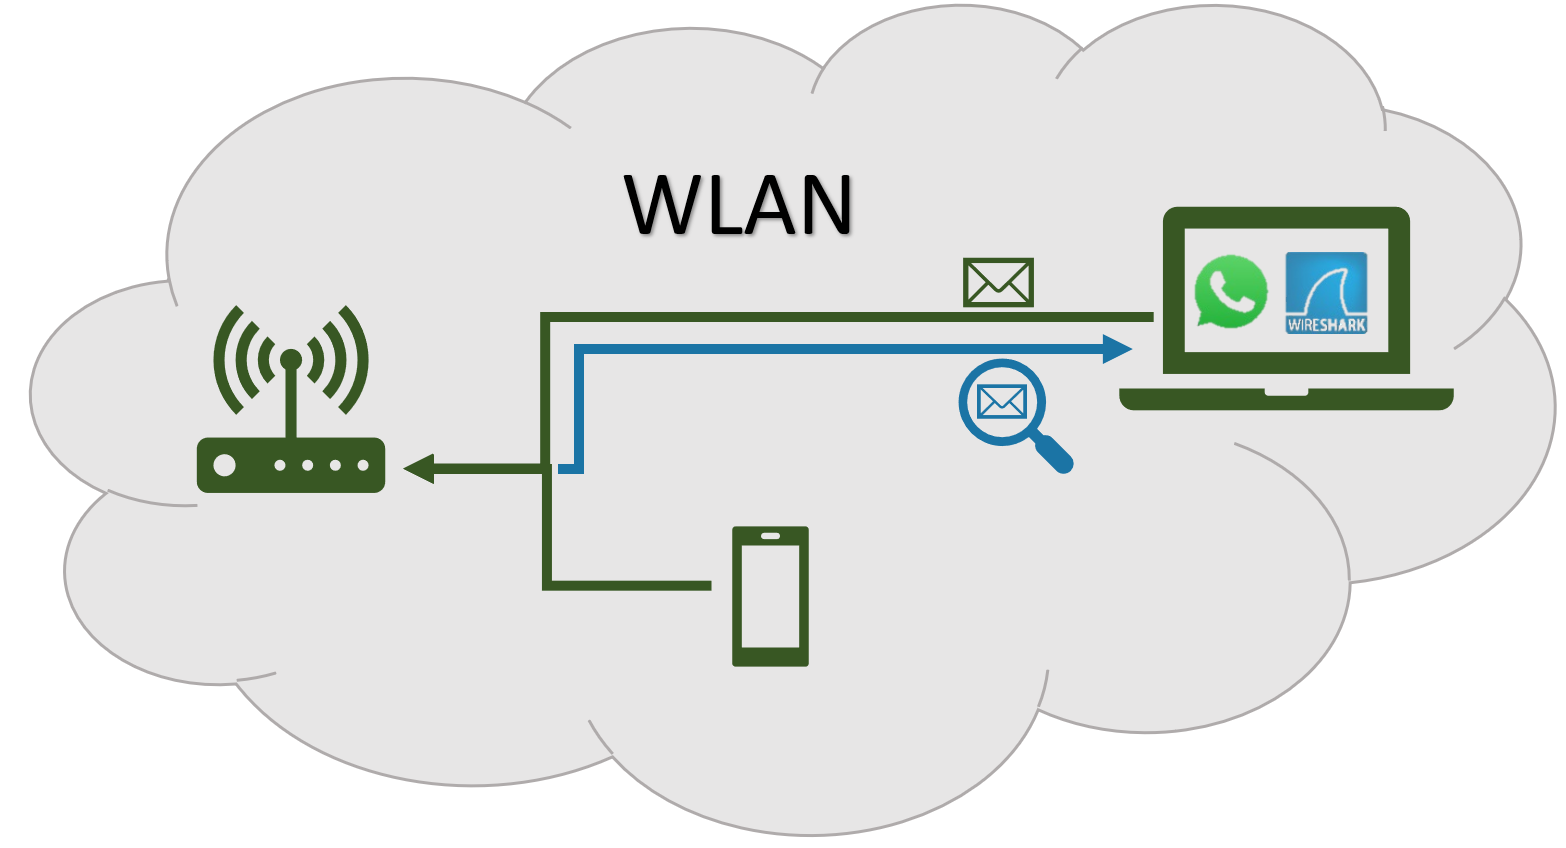
\includegraphics[width=9cm]{Aufbau}
\end{center}

\begin{description}
    \item \textbf{Laptop}
        \begin{description}
            \item \textit{WebWhatsApp}: 
                Über diesen Laptop wird WebWhatsApp aufgerufen. Der Client ist 
                bereits auf registriert. 
            \item \textit{Wireshark}:
                Zusätzlich ist Wireshark installiert um die gesamte Netzwerkkommunikation
                zu analysieren.
        \end{description}
    \item \textbf{Smartphone}
    \begin{description}
       \item Das Smartphone über das der Laptop Client bei WhatsApp registriert ist, muss
            sich im Internet befinden. In diesem Fall ist es im gleichen WLAN (müsste es aber nicht sein). 
    \end{description}
\end{description}

\subsection{Analyse mit Wireshark}
\subsubsection{Vorgehen und erster Überblick}
Da zunächst noch nicht bekannt ist, welche Pakete von WhatsApp verschickt werden.
Wird das Capturing von Wireshark ohne Capture Filter ausgeführt. Nachteil ist, 
dass dadurch viel zu viele Pakete angezeigt werden z.B. verschiedene Dropbox Jobs. 
Deshalb müssen zunächst die für die WhatsApp-Analyse relevanten Pakete bzw. Streams
gefunden werden. 
Die einfachste Möglichkeit ist es nach der IP-Adresse zu filtern. 
WebWhatsApp verwendet IPv6 und hat die Adresse: \texttt{2a03:2880:f22d:c5:face:b99c:0:167}. 
Mit diesem Display-Filter ist es möglich das 'Client Hello' Paket vom TLS.v3-Handshake zu finden. 

\begin{center}
    
\includegraphics[width=14cm]{ClientHelloTLS}
\end{center}
Dieser SSL-Session kann im Anschluss gefolgt werden. So wird der gesamte SSL-Stream angezeigt.

\begin{center}
    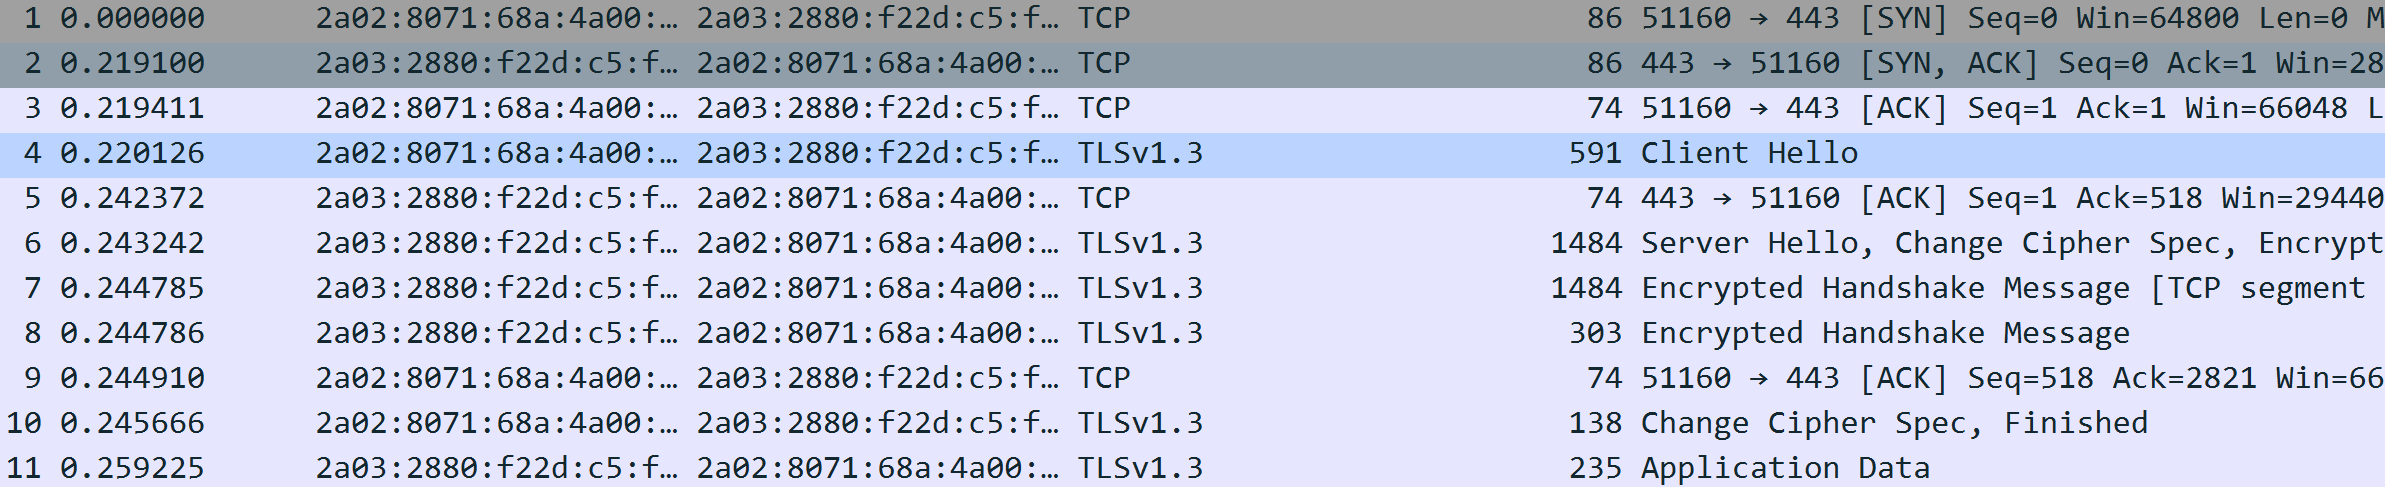
\includegraphics[width=15cm]{WhatsAppFilteredOverview}
\end{center}

In diesem Wireshark-Ausschnitt sind 4 Aktionen sichtbar:
\begin{enumerate}
    \item TCP Handshake
    \item TLSv1.3 Handshake
    \item TLS Cipher-Suite Einigung
    \item Übertragung der Daten von WhatsApp    
\end{enumerate}

Diese einzelnen Aktionen, die notwendig zum Aufbau der Session sind, 
werden im Folgenden genauer analysiert.

\subsubsection{TCP Handshake}
Die ersten drei Pakete des Wireshark-Snippets stellen den TPC Handshake dar.

\begin{center}
    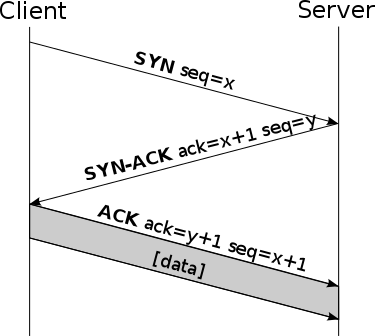
\includegraphics[width=4.5cm]{TCPHandshake0}
\end{center}
Dieser Handshake ist notwendig um eine Verbindung zwischen den beiden Sockets von Client
und Server herzustellen.

\begin{center}
    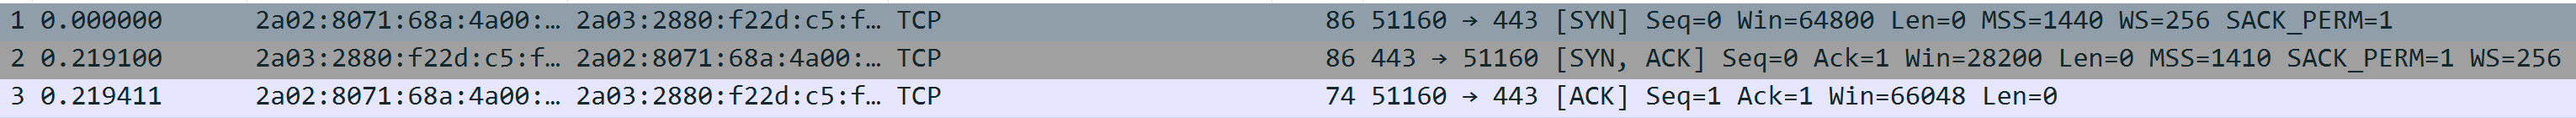
\includegraphics[width=15cm]{TLSHandshake1}
\end{center}
In diesem Wireshark-Snippet ist genau dieser Ablauf zu erkennen.
Wireshark bietet die Möglichkeit, die Pakete in einem Flowchart anzuzeigen. 
Dieser ist für einen Überblick sehr hilfreich.
\begin{center}
    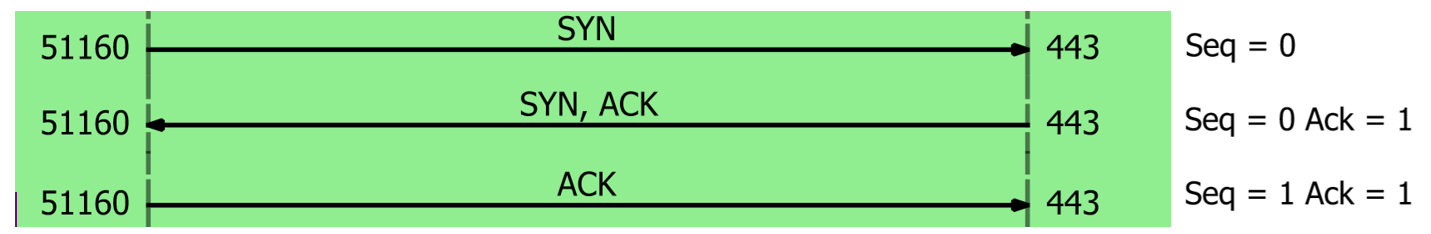
\includegraphics[width=10cm]{TCPHandshakeOverview} 
\end{center}

Zunächst sendet der Laptop (mit WebWhatsApp) das \texttt{SYN-Paket} mit einer Sequenznummer.

\begin{center}
    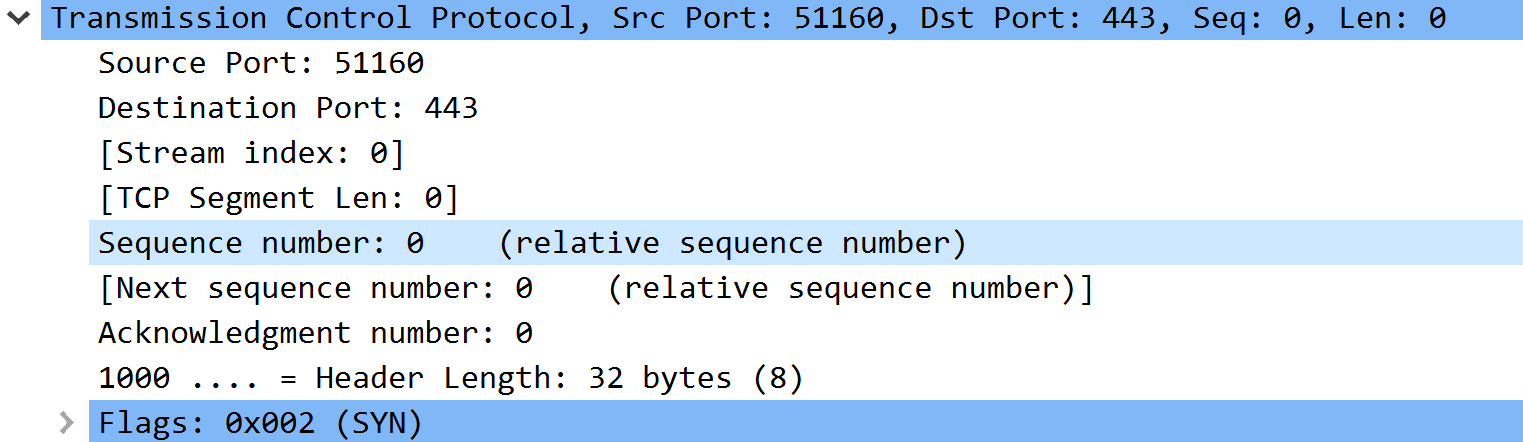
\includegraphics[width=10cm]{TCPHandshake1}
\end{center}

In diesem Fall ist die \texttt{Sequenznummer = 0}
Der Server antwortet mit einem \texttt{SYN-ACK-Paket}.

\begin{center}
    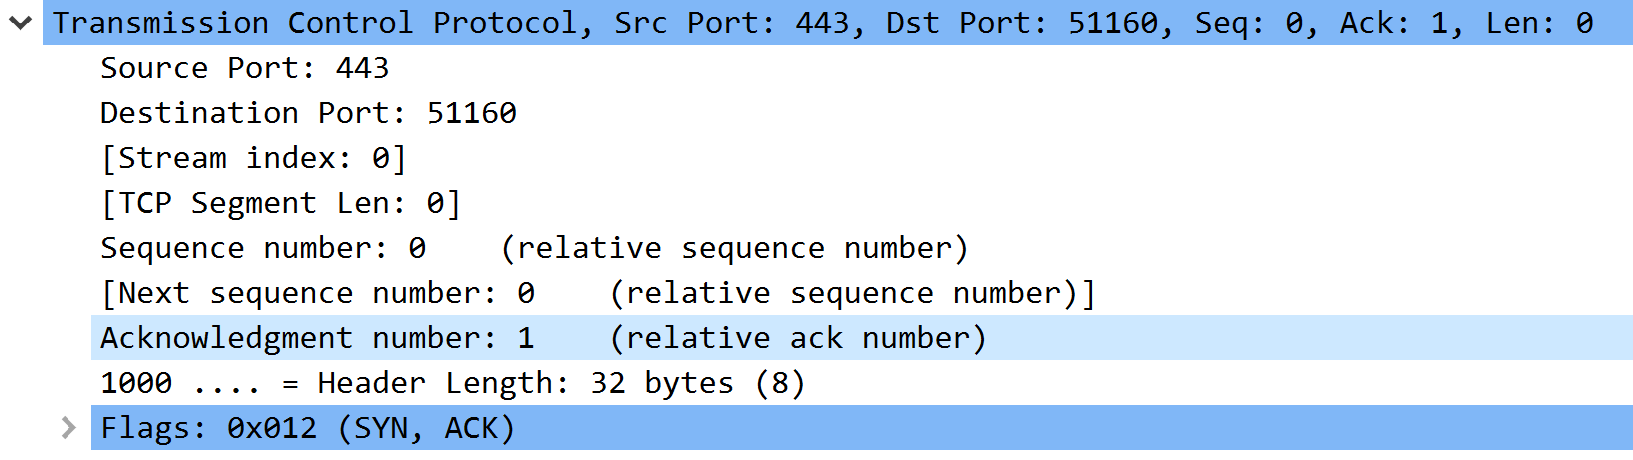
\includegraphics[width=10cm]{TCPHandshake2}
\end{center}

Dort ist die \texttt{Acknowledgementnummer = 1} und eine neue \texttt{Sequenznummer = 0}. 
Zum Abschluss des Handshakes sendet der Client dem Server seinerseits ein \texttt{ACK-Packet}.

\begin{center}
    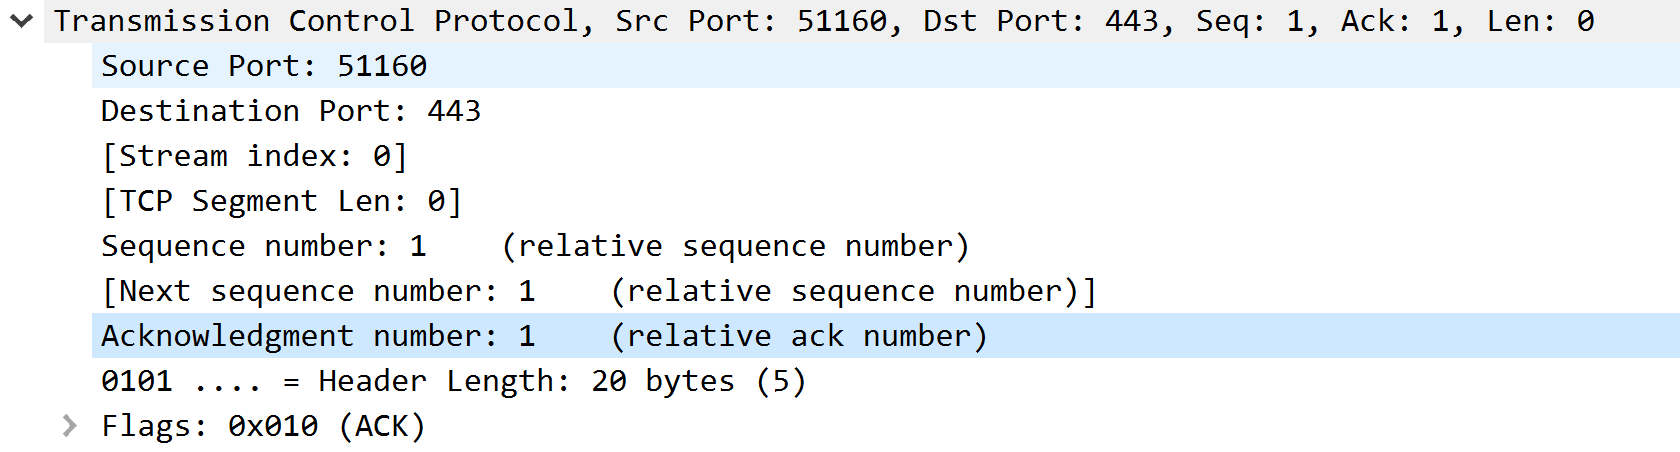
\includegraphics[width=10cm]{TCPHandshake3}
\end{center}

\subsubsection{TLSv1.3 Handshake}
Für den TLSv1.3 Handshake sieht der Flowchart der von Wireshark generiert
wird wie folgt aus.

\begin{center}
    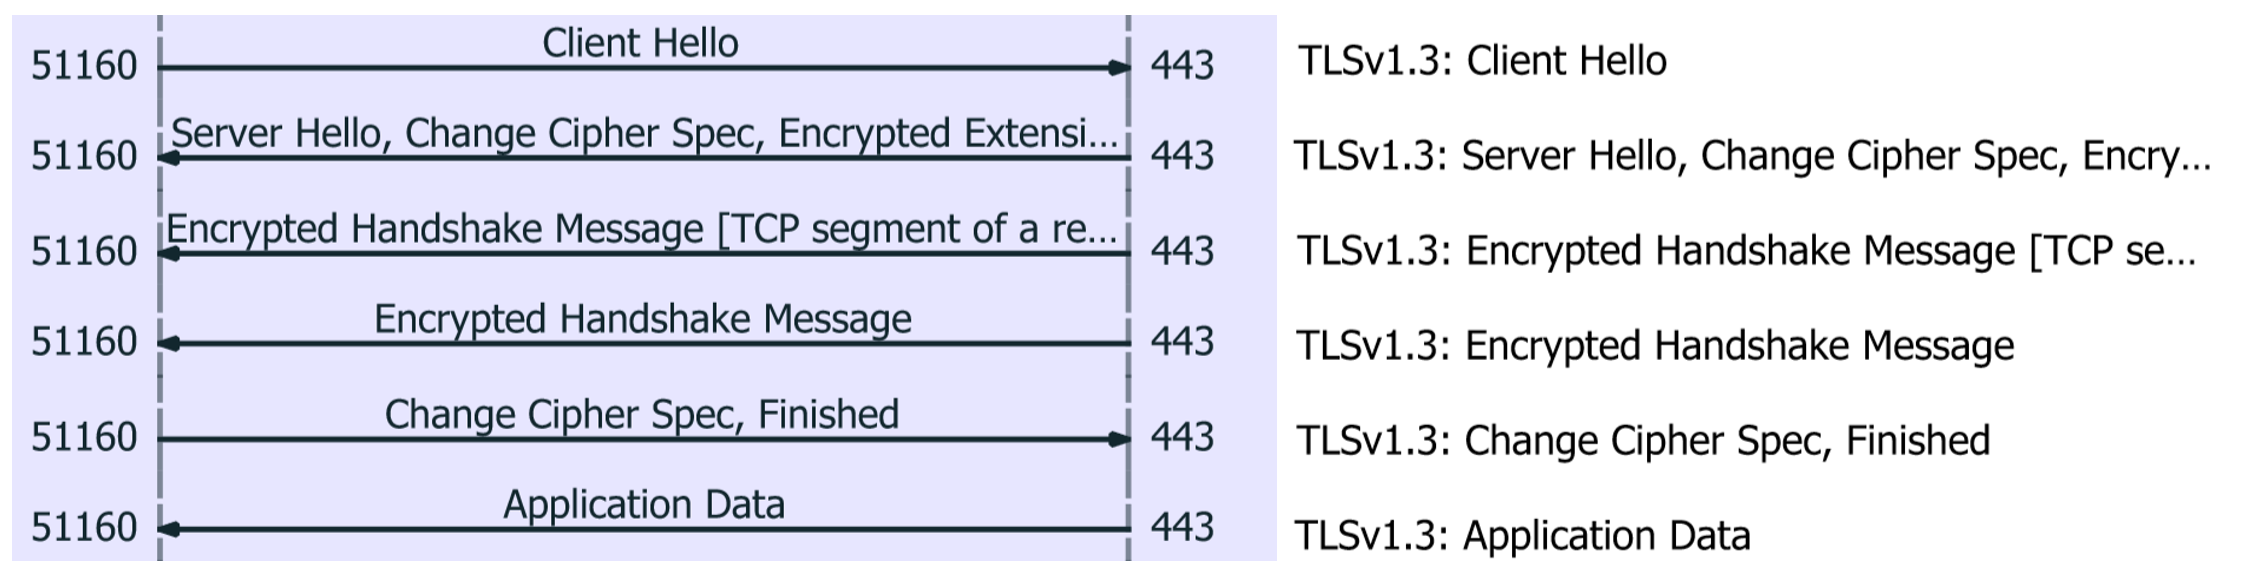
\includegraphics[width=10cm]{TLSHandshakeOverview}
\end{center}

\textbf{Client Hello}\\

\textbf{Sever Hello, Cipher Suite}\\

\textbf{Encrypted Handshake Message}\\

\textbf{Finished}\\

\textbf{Application Data}\\

\subsubsection{Einigen auf Cipher-Suite}
\subsubsection{Übertragung der Application Data}
\section{Fazit}\label{sec:fazit}
Für die Übertragung von Informationen verwendet WhatsApp den neues Stand der Technik. 
Während der Analyse des eigenen WLANs ist deutlich geworden, dass die Pakete von WhatsApp 
die einzigen Pakete waren, die mit TLSv1.3 verschlüsselt wurden. 
Die Ende-zu-Ende-Verschlüsselung der Nachrichten verwendet mit AES und dem Deffie-Hellman Verfahren zum Austausch der SChlüssel
eine sichere Methode für die Datensicherheit. 
WhatsApp behauptet die privaten Schlüssel der Clients nicht zu kennen, diese seien nicht auf den Servern gespeichert, 
sondern lediglich auf den End-Geräten verfügbar. Dies müsste allerdings in einem weiteren 
Projekt analysiert werden. 
Durch die Verschlüsselung und die Verwendung von TLSv1.3 sind bei der Analyse der Pakete nur wenige Informationen 
verfügbar. Zu erkennen sind die Verfahren und Protokolle die WhatsApp verwendet. 
Diese werden allerdings auch von WhatsApp nicht geheimgehalten, denn die Verfahren sind nicht durch ihre Geheimhaltung sicher, sondern durch 
die Geheimhaltung des privaten Schlüssels. WhatsApp hat sich in dem letzten Jahr sehr viel Gedanken bzgl. der Nachrichtenübertragung im Bezug 
auf Sicherheit gemacht und verbessern diese stetig. 

%\printacronyms{}
\printbibliography{}
\end{document}